\documentclass[12pt]{article}


\usepackage{apuntes-estilo}
\usepackage{fancyhdr,lastpage}
\usepackage{color,colortbl}
\usepackage{verbatim}

\def\maketitle{

% Titulo 
 \makeatletter
 {\color{bl} \centering \huge \sc \textbf{
 Periféricos\\ 
\large \vspace*{-8pt} \color{black} Programación de Sistemas Embebidos
 \vspace*{8pt} }\par}
 \makeatother


% Autor
 \makeatletter
 {\centering \small 
 	Departamento de Ingeniería de Computadoras \\
 	Facultad de Informática - Universidad Nacional del Comahue \\
 	\vspace{20pt} }
 \makeatother

}

% Custom headers and footers
\fancyhf{} % clear all header and footer fields
\fancypagestyle{plain}{\fancyhf{}}
  	\pagestyle{fancy}
 	\lhead{\footnotesize Periféricos - Programación de sistemas embebidos}
 	\rhead{\footnotesize \thepage\ }	% ''Page 1 of 2''

\def\ti#1#2{\texttt{#1} & #2 \\ }



\begin{document}

\thispagestyle{empty}
\maketitle
\setlength{\parindent}{0pt}




Además del procesador y memoria, la mayoría de los sistemas embebidos
contienen varios dispositivos de hardware extra. Algunos de estos
dispositivos son específicos a la aplicación, mientras que otros -como los
relojes y puertos seriales- son útiles de una manera general a una gran 
variedad de sistemas distintos.
Los que residen junto con el procesador dentro del mismo chip se los
denomina periféricos internos, u on-chip. Los que se encuentran fuera
del chip donde está el procesador se los denomina de manera opuesta,
es decir, periféricos externos. En este capítulo se detalla la
mayoría de los problemas de software comunes que surgen cuando se programan
periféricos de ambos tipos.

\subsection *{Registros de estado y de control}

La interfaz básica entre un procesador embebido y un dispositivo periférico
es un conjunto de registros de estado y control. Estos registros son parte
del hardware del periférico, y sus ubicaciones, tamaño (en bits) y significado
individuales son característicos de cada dispositivo. Por ejemplo, 
el significado de los bits de los registros de un controlador serial son 
muy diferentes a los
de los contadores o relojes. En esta sección se encuentra explicado la 
manera de manipular el contenido de los registros de estado y control
directamente desde programas en C/C++.

Dependiendo del diseño del procesador y la placa, los dispositivos periféricos
se encuentran localizados en el espacio de memoria del procesador o dentro
del espacio de E/S. De hecho, es común en sistemas embebidos que se incluyan
periféricos de ambos tipos. Se los denomina periféricos mapeados en memoria
y periféricos mapeados en E/S respectivamente. De los dos tipos, los periféricos
mapeados en memoria son los más fáciles de utilizar y por lo tanto su popularidad
aumenta.

Los registros de estado y control de periféricos mapeados en memoria se pueden
parecer a variables comunes en un programa. Por ejemplo, es posible 
declarar un puntero en C a un registro o bloque de registros, 
y establecer
la dirección (valor del puntero) explícitamente. Supongamos el registro
PORTB utilizado en el capítulo 2, el cual es mapeado en memoria en la dirección 
física 0x25. La función toggleLed estudiada en ese capitulo puede ser 
escrita completamente en C, como se muestra a continuación.

\begin{verbatim}
unsigned char * puerto_b = (unsigned char *) 0x25;

void toggleLed(void)
{
    *puerto_b ^= LED_ROJO;    /* Read, xor, and modify. */
}    /* toggleLed() */
\end{verbatim}

Aquí se declara un puntero a un registro de 8 bits y explícitamente se lo
inicializa con  la dirección 0x25. A partir de este momento el puntero al 
registro
trabaja como cualquier puntero a una variable de tipo char de 8 bits.


\subsubsection *{Uso de volatile en C o C++}

Note que existe una diferencia muy importante entre 
registros de dispositivos y variables ordinarias. El contenido de un registro
de dispositivo puede cambiar sin que el programa intervenga o se notifique
del cambio. Esto sucede porque el contenido del registro puede ser modificado
por el hardware del dispositivo. De manera contraria, el contenido de una
variable no cambiará a menos que el programa modifique la misma explícitamente.
Por esa razón, se dice que el contenido de un registro de dispositivo
es volátil, o sujeto a cambiar sin notificación previa.

En C y C++ se debe utilizar la palabra clave volatile cuando se 
declaran punteros a registros de dispositivos.
La misma le indica al compilador que no puede realizar suposiciones acerca
del dato almacenado en esa dirección. Por ejemplo, si el compilador
observa una escritura a una ubicación volátil y luego inmediatamente 
le sigue otra instrucción de escritura a la misma ubicación, el compilador 
no asume  que la primer escritura es innecesaria. En otras palabras, la
palabra clave volatile instruye a la fase de optimización del compilador 
a tratar a esa variable como volátil, y que su conducta no puede ser
predecible en tiempo de compilación.

Prosiguiendo con el ejemplo anterior, se muestra aquí debajo el uso 
de volatile para advertir al compilador acerca del registro PORTB :

\begin{verbatim}
volatile unsigned char * puerto_b = (unsigned char *) 0x25;
\end{verbatim}

Es importante notar que es erróneo interpretar, en esta declaración,
que el puntero en si mismo es volátil. De hecho, el valor de la
variable puerto\_B tendrá el valor 0x25 durante toda la ejecución del programa
(a menos que el valor sea modificado por alguna instrucción del programa, por
supuesto). Mas bien es el dato apuntado el que está sujeto a cambiar
sin que el programa intervenga. Este detalle es muy sutil y es fácilmente
confundible al pensar mucho en el tema. Solamente recuerde que la ubicación
de un registro es fija aunque su contenido podría no serlo. Por lo tanto, si se
utiliza la palabra clave volatile, el compilador asumirá lo mismo.

La principal desventaja de los demás tipos de registros, registros mapeados
a E/S, es que no hay una manera estándar de acceder a ellos desde C o C++. 
Estos registros son únicamente accesibles con la ayuda de instrucciones
de lenguaje máquina especiales. Y estas instrucciones especificas del procesador
no son soportadas por los estándares del lenguaje C o C++. Por lo tanto
es necesario utilizar rutinas de bibliotecas especiales, o código en lenguaje
ensamblador entre lineas, para leer y escribir los registros de un
dispositivo mapeado al espacio de E/S.


\subsection *{La filosofía del controlador de dispositivo}

\fcolorbox{black}{grey}{
\parbox[t]{1.0\linewidth}{ \vspace*{0.4cm}
NOTA: En el diseño de controladores (drivers) de dispositivos se debe
siempre enfocar una meta común : ocultar el hardware completamente.
\vspace*{0.4cm} } }

Cuando se completa un proyecto, el modulo controlador de dispositivo debe 
ser la única
pieza de software en el sistema entero que lee o escribe directamente a los 
registros de estado y control particular de un periférico. Además, si el 
dispositivo 
genera interrupciones, la rutina de servicio de interrupciones que 
atiende las mismas debe ser una parte integral del controlador de dispositivo.
En esta sección se explica el por qué se recomienda esta filosofía y cómo
puede ser lograda.

Por supuesto, intentar ocultar el hardware completamente es difícil. Sea cual
sea la interfaz de programación que se seleccione siempre reflejará las
características generales del dispositivo. Esa característica es esperada
e inevitable. La meta tiene que ser que la interfaz de programación
desarrollada no debería necesitar cambios si el periférico final es reemplazado
con otro de su misma clase general. Por ejemplo, todos los dispositivos de memoria
Flash comparten los conceptos de sectores (aunque el tamaño del sector
puede diferir entre chips). Una operación de borrado puede ser realizada
únicamente en un sector entero, y una vez eliminado, bytes individuales
de palabras pueden ser reescritos. Por lo tanto, la interfaz desarrollada
en un controlador de memoria Flash debería ser útil con cualquier
dispositivo de memoria similar.

Los controladores de dispositivos para sistemas embebidos son bastante
diferentes con respecto a los controladores para estaciones de trabajo.
En una computadora general, los controladores de dispositivos están
desarrollados con el objetivo de satisfacer los requerimientos del sistema
operativo. Por ejemplo, los sistema operativos de PC usualmente imponen
requerimientos estrictos en la interfaz de software entre el SO y una
placa de red. El controlador de dispositivo para una placa de red particular
debe cumplir con la interfaz de software, sin importar las características
y capacidades del hardware subyacente. Los programas de aplicación que 
necesitan utilizar la placa de red están forzados a utilizar la API
de red provista por el sistema operativo, y no tienen acceso directo a la
placa en si misma. En este caso la meta de ocultar el hardware completamente
es alcanzada más fácilmente.

En contraste, el software de aplicación en un sistema embebido  puede acceder al
hardware directamente. De hecho, debido a que todo el software es
vinculado en conjunto en una imagen binaria individual, raramente existe
una
distinción entre la aplicación, sistema operativo, y controladores
de dispositivos.
Esta distinción, como así también la aplicación de restricciones de acceso 
al hardware,
son meramente responsabilidades de los desarrolladores de software embebido.
Ambas son decisiones de diseño que los desarrolladores deben realizar
concienzudamente. En otras palabras, los programadores de software 
embebido pueden tener más flexibilidad en el diseño del software
que sus pares no embebidos (lo cual no significa que esto sea
una ventaja).

Los beneficios de un buen diseño de controlador de dispositivo son tres.
Primero, debido a la modularización, la estructura de todo el software
se comprende más fácilmente. Segundo, como hay únicamente un modulo 
que interactúa directamente con los registros del periférico, el estado
del hardware puede ser verificado mas precisamente. Finalmente, el ultimo 
beneficio pero no por eso menos importante, los cambios en el software que
resultan de los cambios en el hardware están localizados en el controlador
de dispositivo. Todos estos beneficios ayudan a reducir el numero total
de errores en el software embebido.
Pero, se debe estar dispuesto a
poner un poco de esfuerzo extra al momento del diseño con el fin de 
alcanzar estos beneficios.

Si acuerda con esta filosofía de ocultar todas las especificaciones del hardware
e interacciones dentro del controlador de dispositivo usualmente debe 
implementar y utilizar los cinco componentes de la lista presentada a continuación.
Para realizar una implementación del controlador lo más simple e incremental
como sea posible, se debería desarrollar estos elementos en el orden
presentado.

1. Una estructura de datos que se superpone (overlay) a los registros de estado
y de control del dispositivo mapeados en memoria.

El primer paso en el proceso de desarrollo del driver es crear una estructura
(struct), al estilo del lenguaje C, que represente de manera exacta los registros
mapeados en memoria del dispositivo. Generalmente, se necesita estudiar
la hoja de datos del periférico y crear una tabla para los registros
de estado y de control junto con sus desplazamientos (en memoria).
Entonces, comenzando con el registro con la dirección más baja, se 
va completando la tabla de la estructura. Si existen ubicaciones no 
utilizada o reservada entre los registros se puede ubicar variables
vacías para ocupar espacio adicional acorde.

Un ejemplo de una estructura de datos del estilo se presenta a continuación.
La misma describe los registros del hardware serial USART presente dentro
del atmega328p. El dispositivo tiene seis registros, dispuestos como se muestra
a continuación en la estructura de datos serial\_st. Cada registro es de 
8 bits y deberían ser manipulados como un unsigned char.

\begin{verbatim}
struct serial_st
{
    uint8_t data_es;	/* udr0 i/o data */
    uint6_t baud_rate_h;    /* ubrr0h baud rate high */
    uint8_t baud_rate_l;    /* ubrr0l baud rate low */;
    uint8_t _reserved;    /* espacio sin utilizar */
    uint8_t status_control_c;    /* ucsr0c USART Control and Status C */
    uint8_t status_control_b;    /* ucsr0b USART Control and Status B */
    uint8_t status_control_a;    /* ucsr0a USART Control and Status A */
}
\end{verbatim}


Para leer y escribir bits individuales mas fácilmente es una practica común
definir mascaras de bits para usos comunes:

\begin{verbatim}
#define RECEIVER_ENABLE 0x10        /* RXEN0 Habilitar la recepcion */
#define TRANSMITTER_ENABLE 0x08     /* TXEN0 Habilitar la transmicion */
#define CHARACTER_SIZE_0 0x20       /* UCSZ00 Numero de bits del dato de e/s */
#define CHARACTER_SIZE_1 0x40       /* UCSZ01 Numero de bits del dato de e/s */
#define READY_TO_READ 0x80          /* RXC0 Dato listo para leer */
#define READY_TO_WRITE 0x20         /* UDRE0 Buffer vacio listo para escribir */
\end{verbatim}


2. Un conjunto de variables para mantener el estado actual del hardware
y del controlador del dispositivo

El segundo paso en el proceso de desarrollo del controlador es definir
qué variables se necesitan para mantener el estado del hardware y 
del controlador del dispositivo. Por ejemplo, en el caso del controlador 
serial probablemente se necesita conocer si el
hardware ha sido inicializado.

Algunos controladores de dispositivos crean mas de un dispositivo de software.
Esto es un dispositivo puramente lógico, que es implementado por encima
del hardware periférico básico. Por ejemplo, es fácil imaginar
que mas de un reloj por software puede ser implementado desde una
unidad contador/reloj (timer/counter). El dispositivo contador/reloj se configura
para generar un tick de reloj periódico, y el controlador de dispositivo
gestionaría un conjunto de relojes por software de varias duraciones,
manteniendo información del estado de cada reloj software.

3. Una rutina para inicializar el hardware a un estado conocido

Una vez que se conoce como mantener el estado de los dispositivos 
lógicos y físicos es momento de comenzar a escribir las funciones que 
interactúan y controlan el dispositivo. Es conveniente comenzar 
con la rutina de inicialización del hardware. Además, necesitará
esa rutina primero, y esa es una buena manera de entender como interactuar
con el dispositivo.

4. Un conjunto de rutinas que, en su conjunto, presentan una API 
a los usuarios del controlador de dispositivo

Luego de que se haya inicializado el dispositivo correctamente es
momento de agregar otras funcionalidades al controlador. Es en este
paso en donde se deben establecer los nombres y propósitos de varias 
rutinas, como así también sus respectivos parámetros y valores devueltos.
Una vez definidas es el momento de implementar cada función junto
con un caso de test mínimo. Se presentan ejemplos de tales rutinas
en la siguiente sección.

5. Una o varias rutinas de atención de interrupciones

Es conveniente diseñar, implementar y verificar la mayoría de las rutinas
del controlador de dispositivo antes de habilitar las interrupciones.
Encontrar el origen de los problemas relacionados con las interrupciones
es muy difícil. Además, si existen errores (bugs) en otros módulos
controladores, la búsqueda del problema relacionado con las interrupciones
puede no tener fin. Por lo que es mejor utilizar 
E/S programada (polling) primero, para obtener el controlador funcionando.
De esta manera se comprenderá cómo trabaja el dispositivo (y que 
realmente esté funcionando) cuando se comienza a buscar la fuente
de los problemas relacionados con las interrupciones. Finalmente, cabe
decir que, desafortunadamente, suele haber casi siempre problemas 
relacionados con las interrupciones cuando se implementa el control por 
software de las mismas.

\subsection *{Un controlador de dispositivo serial}

El ejemplo de controlador de dispositivo que se presenta está diseñado
para controlar un puerto serial. El hardware para este controlador
de dispositivo utiliza un periférico UART 
(pronunciado 'you-art' y es el acrónimo de
Universal Asynchronous Receiver Transmitter) que se encuentra en el atmega328p.
Un UART es un componente que recibe y envía de manera serial y asincrónica
información. Asincrónico significa que el dato puede llegar en cualquier
momento, similar a la entrada provista por un teclado. Un UART acepta
un byte de forma paralela desde el procesador, el cual es serializado,
y cada bit es transmitido en el momento apropiado. La recepción trabaja
a la inversa.

Es importante aclarar que el atmega328p tiene en su chip un USART (Universal Synchronous and Asynchronous serial Receiver and Transmitter) que puede trabajar
en modo sincrónico, y también, como periférico SPI maestro. En nuestro
controlador utilizamos únicamente el modo asincrónico no SPI.

Antes de diseñar y desarrollar el controlador de dispositivo 
es importante entender el diagrama de bloques del hardware -el cual
presenta cómo las señales van y vienen desde el periférico al exterior del mismo.
Típicamente, esta tarea se logra  observando las porciones relevantes de los
esquemáticos, y leyendo las hojas de datos de los diferentes integrados.
Un diagrama de bloques para el puerto serial se muestra en la Figura \ref{fig:usart-block}.

\begin{figure}
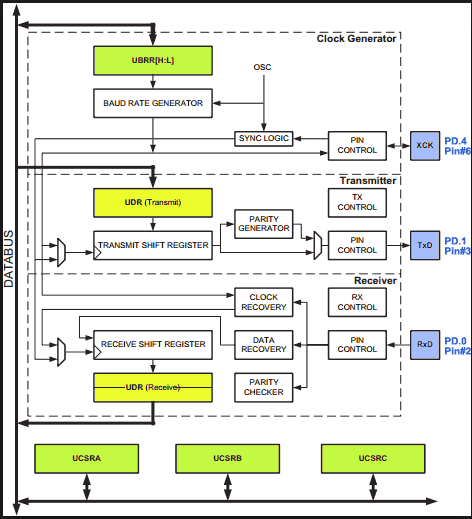
\includegraphics[width=\linewidth]{usart-block.png}
\caption{Diagrama de bloques del USART en el atmega328p.}
\label{fig:usart-block}
\end{figure}


Qué integrados se necesitan programar para controlar el periférico?
Para este ejemplo de controlador serial únicamente nos enfocamos
en el USART. La información de los registros está localizada en la hoja
de datos del microcontrolador atmega328p. Mientras se lee esta información
se debe tener en cuenta que la meta es entender varios conceptos. Algunos
de ellos son :
- La estructura de los registros para controlar el periférico, que incluye
el cómo configurar las comunicaciones y como obtener y enviar
datos desde el periférico.
- Las direcciones de memoria de los registros de estado y de control.
- El método que se debe utilizar para la operación del periférico (E/S 
programada o con interrupciones).
- Si se utilizan interrupciones entonces se debe entender bajo qué condiciones
se producen las interrupciones, cómo el controlador de software se informa
de las mismas, y cómo debe atenderlas.

Se debe obtener un control claro sobre lo que necesita el controlador 
de dispositivo para llevar adelante la tarea del periférico dentro del
sistema. Una vez que estos pasos iniciales están completos, 
se puede continuar con la tarea de escribir el software del controlador
para el dispositivo.

/subsubsection *{Registros interfaz}

El primer paso para el controlador de dispositivo serial es definir
la interfaz de los registros. Para este ejemplo, utilizamos
una estructura que se superponga a los registros del USART, los cuales
están mapeados a memoria. La estructura uart\_t se muestra a continuación :


\begin{verbatim}
typedef struct 
{
    uint8_t data_es;	/* udr0 i/o data */
    uint6_t baud_rate_h;    /* ubrr0h baud rate high */
    uint8_t baud_rate_l;    /* ubrr0l baud rate low */;
    uint8_t _reserved;    /* espacio sin utilizar */
    uint8_t status_control_c;    /* ucsr0c USART Control and Status C */
    uint8_t status_control_b;    /* ucsr0b USART Control and Status B */
    uint8_t status_control_a;    /* ucsr0a USART Control and Status A */
} volatile uart_t
\end{verbatim}

La variable puertoSerial se utiliza para acceder a los registros
en la dirección 0xc6 (que es la dirección mas baja del registro data\_es),
y es definida así :

\begin{verbatim}
uart_t *puertoSerial = (uart_t *) (0xc6);
\end{verbatim}


/subsubsection *{Variables de estado}

El siguiente paso es definir variables para mantener el estado actual
del hardware. Se declara entonces, en el ejemplo, una estructura
que contiene los parámetros del controlador serial, llamado serialparams\_t.
También, se crea una variable global que contendrá los valores 
de configuración actual definidos en la estructura anterior.

Una variable más, llamada initialized se define, para mantener el estado 
de si el 
controlador del dispositivo está inicializado o no.

\begin{verbatim}
typedef struct
{
    uint32_t dataBits;
    uint32_t stopBits;
    uint32_t baudRate;
    parity_t parity;
} serialparams_t;

serialparams_t gSerialParams;
\end{verbatim}


/subsubsection *{Rutina de inicialización}

La rutina de inicialización serial\_init configura los parámetros de comunicación
predeterminados para el controlador de dispositivo serial.
Los registros del USART son programados en la rutina serial\_config, el
cual recibe como argumentos los parámetros de la variable gSerialParams.
La variable initialized es utilizada para asegurar que el puerto
serial es configurado únicamente una vez.


FUNCION INIT


/subsubsection *{API del controlador del dispositivo}


Ahora ya es posible incorporar funcionalidad adicional, definiendo otras
funcionas en el controlador del dispositivo serial.
La API para el controlador de dispositivo serial debería tener, al menos,
funciones para enviar y recibir caracteres. Para enviar caracteres
se implementa, en este ejemplo, la función serial\_put\_char, y para recibir
caracteres la función serial\_get\_char;


La función serial\_put\_char espera hasta el que transmisor esté listo, y 
luego envía un caracter individual a través del puerto serial (E/S programada).
La
transmisión es realizada al escribir el dato al registro de datos del USART.
El siguiente código muestra la función serial\_put\_char.

FUNCION 


La función serial\_get\_char debe esperar hasta que un caracter es recibido, y 
luego es posible leer el caracter individual desde el puerto serial. 
Para determinar si un caracter ha sido recibido, se puede verificar
el bit data ready, del registro de estado del USART. El caracter
recibido es devuelto a la función llamadora. 
El siguiente código implementa esta función.

FUNCIOn

Debido a que este controlador de dispositivo serial no utiliza interrupciones
el paso final en la filosofía de controlador de dispositivo (implementar
la rutinas que atienden las interrupciones del controlador de dispositivo)
no se implementa.


/subsubsection *{Verificando (testing) el controlador de dispositivo serial}

Ahora que el controlador de dispositivo está implementado, necesita verificar
que funciona correctamente. Es importante verificar las funciones de la nueva
API de manera individual, 
antes de integrar el controlador dentro del sistema de software.

Para verificar el controlador debe conectar el puerto serial de la placa
arduino pro mini a la PC. Debido a que los pines del puerto serial de la placa
funcionan con lógica ttl, se debe utilizar un adaptador. Un adaptador
común en estos días es el que adapta estos niveles ttl a USB, que toda PC
actual tiene.
Luego de conectar el hardware se necesita un programa "terminal", tal
como minicom, picocom, o screen desde la PC. Ejecute uno de estos programas
y configure el puerto serial del sistema operativo en la PC y la
velocidad de la comunicación, que debe ser la misma que la del driver 
implementado.

La función main demuestra como ejecutar las funcionalidades implementadas
en el controlador del dispositivo.

Primero, el controlador del dispositivo serial es inicializado llamando 
a serial\_init. Luego se envían varios caracteres hacia la PC, para 
verificar la función serial\_put\_char. Si el controlador de dispositivo serial
opera correctamente se obtiene el mensaje 'start' en la pantalla terminal
de la PC.

Finalmente un bucle while es ejecutado, chequeando si un caracter
ha sido recibido (llamando a serial\_get\_char). Si se recibe un caracter
en el puerto serial, este es enviado nuevamente a través de un 'eco'.
Si el usuario presiona 'q' en el programa terminal de la PC el programa
embebido finaliza. De otra manera, el bucle continua y comprueba si otro
caracter de entrada arriba volviendo a realizar el 'eco'.



EJEMPLO MAIN


/subsubsection *{Extendiendo la funcionalidad del controlador del dispositivo serial}


Aunque el controlador es muy básico, tiene funcionalidad como para
escribir una aplicación mínima útil.
Además, el controlador de dispositivo 
presentado permite  aprender acerca de la operación de los UARTs.
La lista a continuación son posibles extensiones que puede realizar
si se desea agregar funcionalidad extra.

\fcolorbox{black}{grey}{
\parbox[t]{1.0\linewidth}{ \vspace*{0.4cm}
NOTA: Mantenga esta lista en mente para otros controladores que desarrolle.
\vspace*{0.4cm} } }

/subsubsection *{Configuración seleccionable}

Se puede cambiar serial\_init para que obtenga parámetros de entrada,
que permita a la aplicación que utiliza el controlador especificar
los parámetros de comunicación iniciales. Por ejemplo, baud rate para
el puerto serial.

Error checking

Es importante para los controladores de hardware realizar un adecuado
chequeo de errores. Por lo que una mejora podría ser definir códigos
de errores (por ejemplo, errores en los parámetros, errores de hardware, etc)
en la API de controlador.
Las funciones del controlador utilizarían estos códigos para devolver
el estado de la operación si existe un error. De esta manera, la aplicación embebida
utilizando el controlador puede realizar acciones de alto nivel con respecto
a fallas, y por ejemplo, reintentar la operación.

APIs adicionales

Agregando serial\_get\_str y serial\_put\_str (el cual requiere buffer de
los datos del receptor y transmisor) podría también ser útil. La implementación
de las funciones de cadenas podrían hacer uso de las funciones
serial\_get\_char y serial\_put\_char, si fuese razonablemente eficiente
hacerlo.

Uso de FIFO

Típicamente, UARTs contienen FIFOs para los datos recibidos y transmitidos.
Utilizando FIFOs agrega buffer a ambos canales de recepción y transmisión,
logrando que el controlador UART  sea mas robusto.

Interrupciones

Implementando interrupciones UART para la recepción y transmisión es
usualmente mejor que utilizar E/S programada. Por ejemplo, si en la función
serial\_get\_char se utiliza interrupciones se eliminaría la necesidad
de que el controlador se quede esperando el caracter entrante. 
Por lo tanto, el software de la aplicación es capaz de realizar
otras tareas mientras se espera que el dato sea recibido. 

/subsubsection *{El diseño del controlador de dispositivos}

La mayoría de los sistemas embebidos tienen mas de un controlador de dispositivo.
De hecho, algunas veces pueden tener muchos controladores. En cuanto
mejore con la experiencia necesita entender la manera en que los
diferentes controladores en el sistema interactúan entre ellos. 
También es importante entender muy bien cómo el software de aplicación 
utiliza los controladores de dispositivo para que pueda diseñar APIs apropiadas
.

También, con respecto al manejo de errores, es necesario tener un buen entendimiento de todo el diseño
del software, para conocer los posibles problemas que pueden surgir.
Algunas áreas a considerar cuando se realiza el diseño de la arquitectura
del software que incluye varios controladores de software son :

Prioridades en las interrupciones

si se utilizan interrupciones en los controladores de dispositivos
de un sistema necesita determinar un conjunto apropiado de niveles
de prioridades.


Uso de recursos

Es importante comprender qué recursos son necesarios para cada controlador.
Por ejemplo, imagine el desarrollo de un controlador ethernet para un 
sistema con muy poca memoria.
Es muy probable que esta limitación afecte al esquema de buffer implementado.
El controlador podría manejar el almacenamiento de unos
pocos paquetes entrantes, el cual afectaría al rendimiento de la 
interfaz ethernet.

Compartir recursos

Debe tener presente que en ciertas situaciones puede tener múltiple
controladores de dispositivos que necesitan acceder a un hardware común 
(tales como pines de E/S) o memoria compartida.
Esto hará difícil localizar errores si el
esquema de divisiones de responsabilidades y uso de recursos
no se piensa a fondo antes.





\section*{Referencias}

Michael Barr. Programming Embedded Systems in C and C++ 1st Edition. ISBN-13: 978-1565923546
ISBN-10: 1565923545. O'Reilly Media; 1 edition (February 9, 1999)

\subsection*{Licencia y notas de la traducción}

Este apunte es una traducción del libro de referencia, para
ser utilizado como apunte en la materia de grado
'Programación de Sistemas Embebidos' de la Facultad de Informática,
Universidad Nacional del Comahue.
Se han realizado modificaciones
al contenido para aclarar ciertos detalles o agregar partes nuevas.
 También se han
modificado todos los archivos fuentes de código, ya que fueron
portados a la plataforma Atmel atmega328.

Autores : \\
Rafael Ignacio Zurita ({\tt rafa@fi.uncoma.edu.ar}) \\
Rodolfo del Castillo ({\tt rdc@fi.uncoma.edu.ar})

\fcolorbox{black}{grey}{
\parbox[t]{1.0\linewidth}{ \vspace*{0.4cm}
Esta es una obra derivada del libro de referencia que aún NO ha obtenido permiso de publicación.
\vspace*{0.4cm} } }


\include{licGASL}

\end{document}
 
